\section{Future Work}
\label{sec:future}

Our experience of using deliberative techniques in a highly
inter-disciplinary environment for targeted marine science
applications has shown the need and applicability of such novel
algorithms and methods. In addition to augmenting traditional AUV
surveys more advanced Lagrangian observations, mixed-initiative
methods, our colleagues at MBARI have understood the longer term
implications of our work. Our current and consequently future efforts
are therefore grounded in important science problems in an operational
oceanographic setting.

\begin{figure}[h]
  \centering
  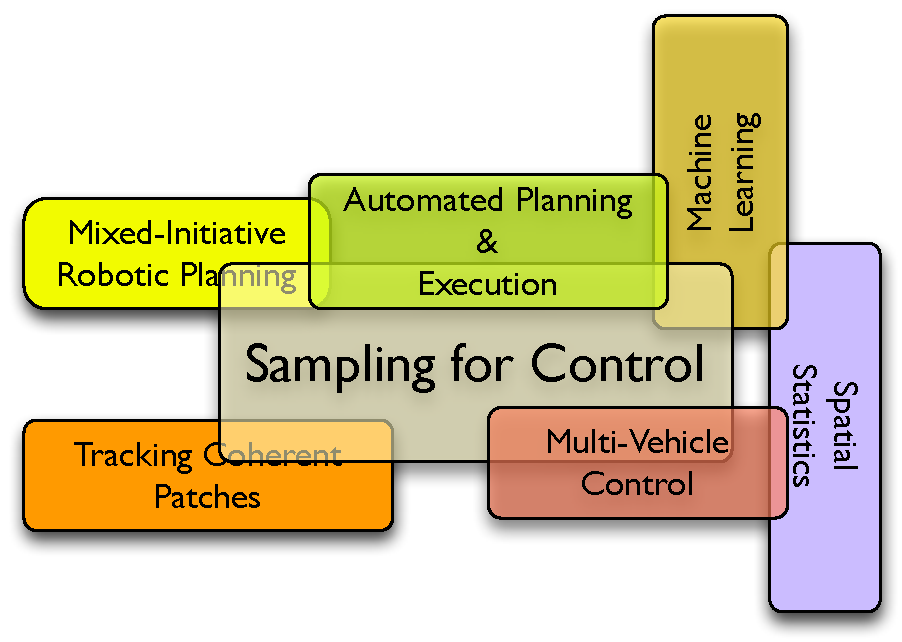
\includegraphics[scale=0.45]{figs/autonomy-topics.pdf}
  \caption{\small Overlapping topics in our research in deliberation
    and autonomy with sampling the dominant theme.}
  \label{fig:topics}
\end{figure}

The core of our problem domain for \can has been towards Sampling. In
large part given the spatial and temporal scales of the
bio-geochemical processes we are interested in in this project, it is
imperative that a key direction is in formulating a multi-robot
adaptive sampling problem. In this context while superficially \rx can
be considered as a multi-agent system and could therefore imply a
direct extension, sporadic communication with high-latencies in
surface communication, not to mention low throughput acoustic
communications imply that the extension of \rx for distributed
applications is non-trivial. Further, in order to efficiently execute
coordinated observation of ocean processes with multiple autonomous
sensing platforms, significant methodological as well as technical
challenges must be addressed. We are working towards a systematic
approach of using \rx as a backend planner for \can field
experiments. The expectation is that \od users will plan initially
individual vehicle surveys which are variants of standard
straight-line transects. Lessons learned with human planners in the
loop will be used towards planning larger surveys, also with simple
fixed transects but using vehicle capabilities in ontologies similar
to \cite{patron09}. Apportioning the planning task between shore-side
components with substantial contextual information and compute power
with robots with in-situ reasoning capabilities a la \rx is a
challenge and an open research problem. Fig. \ref{fig:topics} shows
what we believe is the scope and influence of the different topic
areas we are focusing on.

Partitioned inference and decision-making within \rx also lends itself
to graceful system degradation, making the overall approach effective
towards increased robustness. There are two outstanding diagnosis and
failure recovery challenges that we need to address; the first has to
do with methodology related to model design of the instrument payload
for a highly modular and configurable vehicle; this is local to a
reactor. Doing so would enable (as a first step) using systematic
Fault Diagnosis, Isolation and Recovery (FDIR) algorithms as
demonstrated in the \texttt{RAX} experiment
\cite{williams96,mus98,williams97} and more recently on an AUV by
Dearden and others \cite{wang09,ernits10,dearden11}. The second
challenge has to implementing a policy within the \rx framework that
explicitly deals with recovery since controller failure can be
distributed across reactors. Since reactors are hierarchical in their
relationship to one another, their well defined dependencies allow
them to be removed from an agent systematically. Reactors more
abstract in scope can be removed before those which are less abstract
(and closer to the hardware). In the event a Navigation reactor, for
example, has a fault, it can be removed safely with lower level
functionalities (such as those in the executive). When the Navigator
is removed, it will recursively remove more abstract reactors (such as
a Mission Manager) that depend on it. Such a safety feature then
allows the system designers to ensure that early on they can invest
more in ensuring that reactors lower in the hierarchy are robust and
potentially formally verified. It also means that there is a safe and
sure way to take control of the vehicle at any level within the
reactors hierarchy; as long as low level reactors are still active one
will always been able to send goals/commands to them and execute what
are traditionally known as runout sequences (or clean up scripts).

Feature recognition for Sampling is a general research thrust; however
it has specific relevance in the context of \rx and AUV control. As
noted in Section \ref{sec:results} we have already demonstrated
Machine Learning techniques for recognition of select features in the
coastal ocean. A principal challenge that remains is that of obtaining
expert labeled data for any supervised or semi-supervised learning
methods.  While supervised techniques for learning classifiers such as
decision trees (\cite{Quinlan93-dtrees}), instance-based
classification (\cite{Aha-ibl-ml91}), Bayesian classifiers
(\cite{Jensen2001-BNetworks}) and artificial neural networks
(\cite{ANNsurvey-2000}) are popular, given the vast amount of data
available and poor understanding of correlation between physical and
biogeochemical variables in the coastal ocean, our work on INLs
\cite{mcgann08d,ryan10} and reliance on a oceanographic expert has
shown that scaling to different problems remains problematic. This is
a prime motivation to move towards more semi-supervised methods such
as \cite{kumar11,sergio12}. With the advent of the \od however,
another direction our research is taking us is in Recommender systems
\cite{Adomavicius05} as noted in Section \ref{sec:results}. We are
working to design and deploy software infrastructure that will learn
from user tagged data. To do so, we will use tagging techniques
similar to what users of commercial image sharing sites like Flickr
and Picassa do, to learn the context of the data (including remote
sensing). In addition, the \od will integrate statistical Machine
Learning techniques with incoming asynchronous data stream obtained by
sensors and platforms. Identification models will be based on existing
training sets for INLs and plumes; models for other features of
scientific interests driven by \can requirements will be built in
addition. Existing AUV archives for instance provide sufficient data
for a learning base for a range of features of interest to \can; in
addition we will build software that will learn to incorporate
incoming data streams to provide an existence proof of a feature of
interest. 

Many aspect remain to be fully explored in how to improve \rx and its
integration with \eu. We present here  few of these that we consider
as important in order to improve \rx abilities and reduce the
engineering required to circonvey them.

One of them is related to the dispatchability of
the {\em external} part of the plan \cite{mus98a}. While we were able
to limit its impact so far by adding extra controls inside the \eu
model we know that it can be impoved. For example by analyzing the
plan structure we dshould be able to distinguish part of the plan that
contribute to a  reactor goal -- which often needs to be dispatched
as early as possible -- to other tokens describing the world evolution
for which it can be preferrable to dispatch as late as needed. Being
able to distinguish these two kinds of tokens should largely improve
the quality of the overal agent behavior while avoiding to add extra
complexity on every reactor models. 

At the architecture level we would like to take full benefits of the
reactor graph structure maintained by the agent and how to take full
benefits. One aspect, we need to improve further is the ability to
alter this graph dynamically by creating new reactors or new timeline
connections. Offering such abilty would allow to provide better
reovery mechanism after one reactor has failed to sunchronize by the 
agent. For example, one alternate reactor could take ownership of the
timelines left invalid by the destruction of the faulty reactor. This
would allow to dimplement in atrasnparent way components
redudancy. Still, even though our implementation already allow such
mechanism we do not provide yet this at \rx API level as we need to
ensure that this kind of dynamic alteration of the graph can be done
wothout breaking our current assumptions both at \rx level and \eu
level.

More specifically to \eu level we would like to improve \rx
integration of \eu ability to deliberate about resources. More
specifically we need to ba able to update resource level as 
modeled by \eu based on \rx observation.  As of today the 
support of resource is limited inside the \eu solver and there's no
direct way for \rx to update them dynamically based on recent
observations. This result on a potential discrepeancy between measured
given by, for example, the battery as modeled in \eu and the current
battery level as read in a \rx timeline. Finding an automated way to
link these two constructs would allow the plan to dynamically readapt
when these two values differs -- for example if the vehicle looses a
battery bank during a mission.



% multi-vehicle control
% sampling
% diagnosis and recovery
% feature recognition
% scalable architecture for missions





%%% Local Variables: 
%%% mode: latex
%%% TeX-master: "setobook"
%%% End: 
